\section{Progettazione}
\subsection{XML e XMLSchema}
Si è scelto di adottare XMLSchema al posto di DTD come linguaggio per descrivere la struttura dei file XML perchè più espressivo, e a fini propedeutici, essendo più complesso. Di seguito verranno spiegate alcune scelte riguardanti la struttura.

\paragraph{Scarso utilizzo degli attributi}

I motivi per cui gli attributi sono poco presenti sono tre:
\begin{itemize}
\item Un elemento è maggiormente estendibile rispetto ad un attributo;
\item Un attributo viene utilizzato per descrivere metadati, mentre i dati in se sono inseriti negli elementi;
\end{itemize}

\paragraph{Formato della data}
In molti file è richiesta una data. Si è scelto di salvare tale data in modo esteso, suddividendo l'elemento data in sottoelementi, cosi facendo è possibile indicare dei range di valore accettabili per giorno, mese ed anno. 
Mese viene scritto in lettere e non come numero, si è quindi applicata una \emph{restriction}, partendo da string si accettano solo le stringhe equivalenti ai mesi.
Non è stato utilizzato il tipo \emph{Data} offerto da XMLSchema per evitare di dover utilizzare il formato americano.
Per il tempo è invece stato utilizzato \emph{Data}, precisamente nel file log.xml.

\paragraph{Elementi opzionali}
Nel file riguardante il menù sono presenti elementi non obbligatori. Nel caso di elementi semplici si è scelto di utilizzare l'attributo nillable="true" per indicare che tale elemento è opzionale. Nel file XML dunque l'elemento dovrà sempre essere presente, e nel caso in cui non lo si voglia definire vi si assegnerà xsi:nil="true".  
Nel caso di elementi complessi si è scelto di utilizzare l'attributo minOccurs="0" che permette di non inerire l'elemento nel file XML. Tale scelta è stata fatta per rendere più leggibili i file XML, che risulterebbero altrimenti appesantiti.\\ \\
Questi approcci sono necessari in quanto lasciare semplicemente vuoto l'elemento comporterà un errore di validazione, tranne che per gli elementi di tipo stringa.

\paragraph{Modello adottato}
Il modello adottato è \emph{Bambole russe} in quanto non si è ritenuto il riutilizzo del codice di primaria importanza.
Non si è aderito a tale modello solamente nel file menu.xsd. Questo perchè sono presenti quattro elementi (antipasti, primi, secondi, dessert) tutti con la stessa struttura interna, si è quindi dato un nome al tipo e lo si è messo esterno.

%\section{Il nostro menu e JQuery}
%La pagina \emph{il nostro menu} ha come obbiettivo visualizzare il menu proposto dal ristorante.
%Per rendere più pulita e piacevole la visualizzazione si è messo il contenuto all'interno di vari div (uno per portata) non visibili.
%Cliccando sulla portata verranno visualizzati i relativi piatti e cliccando normalmente verranno nuovamente nascosti.
%Questa tecnica è stata utilizzata nei css per desktop, tablet e smartphone. 
%Per la stampa l'intero menù è stato reso visibile.
%L'accessibilità è garantita da due fattori:
%\begin{itemize}
%\item I div sono nascosti tramite una classe avente il seguente codice, che garantisce la lettura del contenuto da parte dello screen reader
%\begin{lstlisting}
%	position: absolute; 
%	overflow:hidden; 
%	height:0;
%\end{lstlisting}
%\item La classe è applicata ai div tramite JQuery. In tal modo se il browser non supporta javascript, o esso è disabilitato il contenuto resta accessibile.
%\end{itemize}
\subsection{Social}
In ogni pagina, con particolare risalto nella pagina contattaci, è stato reso disponibile un link a Facebook Twitter, Google plus e TripAdvisor. Le motivazioni sono spiegate nella sezione Abstract.
I link non portano a nessuna pagina, in quanto al momento tali pagine non sono presenti, ma verranno create non appena il sito verà accettato e reso pubblico.

\subsection{Contattaci}
La pagina contatti.html permette tramite la compilazione di un form di inviare una mail ai gestori del ristorante.
Si tratta di un modo semplice e veloce per comunicare, e non richiede all'utente di dover accedere al proprio account email. 
In questo momento l'invio della mail non funziona in quanto non è permesso dai server universitari, e la pressione del bottone invia non fa nulla.

\subsection{Sezione d' amministrazione}
In questa sezione sarà possibile accedere solamente dopo aver effettuato la login nell' apposita pagina e qualora si tenti di accedere a questa sezione senza essere autenticati si verrà reindirizzati alla home page del sito. Sarà anche presente in ogni pagina un menu laterale per navigare tra le varie pagine di amministrazione e per tornare alla sezione pubblica.
\paragraph{Dashboard}
Questa sarà la pagina a cui si verrà reindirizzati una volta effettuata la log in, qui ci verrà fornito un messaggio che ci avvertirà con che account siamo loggati e sotto di esso sarà presente una \emph{tabella di log} che avviserà l' amministratore delle ultime azioni effettuate dagli amministratori del sito quali ad esempio l' inserimento di un nuovo evento, l' eliminazione o l' aggiunta di foto segnalando la data e l' ora di tali modifiche.
\paragraph{Modifica photogallery}
In questa sezione verrà data la possibilità all' amministratore di aggiungere nuove immagini alla galleria e modificare i dati di un' immagine quali nome, testo alternativo e titolo, di un immagine preesistente. Sono stati implementati dei controlli per non permettere il submit del form qualora ci sia uno o più campi lasciati vuoti. Inoltre appena l' amministratore inserirà il link all' immagine da caricare, verrà fornita un' anteprima della stessa migliorando l' esperienza dell 'amministratore.
\paragraph{Inserimento nuovo evento}
Qui l' amministratore potrà creare un nuovo evento fornendone il titolo, la descrizione, il costo del menu, la data a cui si riferisce l'evento e le portate che lo compongono. Tutti questi elementi sono obbligatori, e come tali qualora si cerchi di eseguire l' input di tale form, i campi vuoti verranno evidenziati all' amministratore con un' aura rossa intorno ad ogni input box vuota e quando si andrà ad inserire un carattere valido, tale aura verrà rimossa.
\subparagraph{Inserimento nuova news}
Qui i campi saranno tutti necessari, quindi l' amministratore dovrà inserire tutti i campi, e qualora cerchi di eseguire il submit in presenza di campi vuoti non verrà permessa tale azione e verranno evidenziati i campi come nelle altre pagine della sezione privata.

\subsection{Perl}

La codifica di script in \texttt{Perl/CGI} è stata implementata per il \texttt{back-end} dell'applicazione, ovvero la parte che si occupa dell'estrazione, manipolazione e popolamento dei dati da visualizzare. Il codice sorgente, per mancanza di tempo, non è stato commentato secondo una norma e può quindi risultare a tratti poco documentato o difficilmente comprensibile. Il gruppo considera la documentazione un punto fondamentale di qualsiasi progetto \textit{software}, soprattutto per la manutenibilità del codice. Purtroppo la ristrettezza dei tempi e la sovrapposizione di altri impegni da parte dei componenti del gruppo ha impedito di seguire rigorosamente questo principio.

Fondamentalmente gli script si dividono in due categorie principali:

\begin{enumerate}

	\item Gli script che si occupano di popolare lo \textit{scope} dei template \texttt{XHMTL} eseguendo quindi operazioni di lettura dal database;
	\item Gli script che si occupano di eseguire operazioni di scrittura sul database e sul filesystem nel caso di immagini.

\end{enumerate}

I moduli o pacchetti \texttt{CPAN} utilizzati negli script sono i seguenti:

\begin{itemize}

	\item \texttt{HTML::Template} come libreria di \textit{templating} per popolare correttamente i file \texttt{.tmpl} presenti;
	\item \texttt{CGI} per il reindirizzamento e il recupero dei parametri;
	\item \texttt{XML::LibXML} per l'interfacciamento con il database XML;
	\item \texttt{CGI::Session} per la creazione, mantenimento ed eliminazione della sessione utente; 
\end{itemize}
Ciascun file \texttt{.tmpl} in particolare possiede il suo script \texttt{.cgi} che si occupa di popolarlo e visualizzarlo correttamente. \\
Di seguito vengono descritti brevemente e in ordine alfabetico tutti gli script presenti:

\begin{itemize}

	\item \texttt{adminLoader.cgi} si occupa di verificare l'esistenza di una sessione utente e di popolare correttamente la home page dell'amministratore, che sostanzialmente sarà una \textit{dashboard} con al suo interno la lista delle ultime azioni effettuate dagli amministratori;
	\item \texttt{deleteEvent.cgi} si occupa di verificare l'esistenza di una sessione utente e di eliminare dal database l'evento indicato dalla \textit{query string};
	\item \texttt{deleteImage.cgi} si occupa di verificare l'esistenza di una sessione utente e di eliminare dal database e dal filesystem l'immagine indicata dalla \textit{query string};
	\item \texttt{deleteNews.cgi} si occupa di verificare l'esistenza di una sessione utente e di eliminare dal database la news indicata dalla \textit{query string};
	\item \texttt{editImage.cgi} si occupa di verificare l'esistenza di una sessione utente e di modificare nel database e nel filesystem l'immagine indicata dalla \textit{query string} con i parametri passati dal form;
	\item \texttt{editImageLoader.cgi} si occupa di verificare l'esistenza di una sessione utente e generare la pagina di modifica dell'immagine indicata dalla \textit{query string};
	\item \texttt{editNews.cgi} si occupa di verificare l'esistenza di una sessione utente e di modificare nel database la news indicata dalla \textit{query string} con i parametri passati dal form;s
	\item \texttt{editNewsLoader.cgi} si occupa di verificare l'esistenza di una sessione utente e di generare la pagina di modifica della news indicata dalla \textit{query string};
	\item \texttt{errorHandler.cgi} si occupa di generare la pagina standard di visualizzazione di un errore, popolandola con i dati prelevati dalla \textit{query string};
	\item \texttt{eventShow.cgi} si occupa di generare la pagina di visualizzazione dell'evento indicato dalla \textit{query string};
	\item \texttt{eventsHandler.cgi} si occupa di verificare l'esistenza di una sessione utente e di generare la pagina amministratore gestione degli eventi;
\item \texttt{eventsLoader.cgi} Si occupa di popolare correttamente la pagina di visualizzazione degli eventi, prendendo tali eventi dal relativo fai xml;
\item \texttt{galleryAdminLoader.cgi} si occupa di verificare l'esistenza di una sessione utente e di generare la pagina di visualizzazione e modifica della galleria;
\item \texttt{galleryLoader.cgi} Si occupa di popolare correttamente la pagina di visualizzazione della galleria, prendendo le immagini dal relativo fai xml;
\item \texttt{insertEvent.cgi} si occupa di verificare l'esistenza di una sessione utente e di generare la pagina di creazione di un evento;
\item \texttt{insertEventLoader.cgi} si occupa di verificare l'esistenza di una sessione utente e di popolare il file;
\item \texttt{insertImage.cgi}  si occupa di verificare l'esistenza di una sessione utente e di popolare con la nuova immagine e relativi attributi il file gallery.xml;
\item \texttt{insertImageLoader.cgi} si occupa di verificare l'esistenza di una sessione utente e di generare la pagina di aggiunta di un'immagine;
\item \texttt{insertNews.cgi} si occupa di verificare l'esistenza di una sessione utente e di popolare con la nuova news il file news.xml;
\item \texttt{insertNewsLoader.cgi} si occupa di verificare l'esistenza di una sessione utente e di generare la pagina di aggiunta di una news;
\item \texttt{login.cgi} Crea una sessione utente se la login è corretta;
\item \texttt{loginView.cgi} Si occupa di generare la pagina necessaria ad effettuare la login.
\item \texttt{logout.cgi} Esegue il logout distruggendo la sessione utente presente.
\item \texttt{menuLoader.cgi} Si occupa di popolare correttamente la pagina di visualizzazione del menu, prendendo le immagini dal relativo fai xml;
\item \texttt{newsHandler.cgi} si occupa di verificare l'esistenza di una sessione utente e digenerare la pagina per la gestione delle news;
\item \texttt{newsLoader.cgi} Si occupa di popolare correttamente la pagina di visualizzazione delle news, prendendo le immagini dal relativo fai xml;.
\end{itemize} 

\section{CSS}

L’obbiettivo principale che ogni programmatore Web si pone nella fase di progettazione della struttura del proprio sito è quello di farne apparire i contenuti nel modo più chiaro ma allo stesso tempo accattivante possibile. Nel realizzare la struttura del sito "Le vecchie credenze" abbiamo quindi puntato ad ottenere un design assolutamente pulito, privo di ogni possibilità di confusione, che permette l' immediata comprensione dei contenuti anche da parte di un utente casuale. 

\subsection{La struttura}
Le principali sezioni che compongono il nostro sito sono  navigation e content.

\paragraph{Navigation}

Questa sezione contiene il banner ufficiale del sito seguito dal menu a lista attraverso il quale è possibile accedere a tutte le pagine attraverso gli appositi link. Questa sezione contiene anche il footer in cui sono presenti le indicazioni necessarie a raggiungere il ristorante e il link alla sezione “Credits”, che contiene alcune informazioni sui progettatori del sito, “Admin” che permette l’accesso alla pagina di amministrazione e i link ai validatori W3C.


\begin{figure}[H]
		\centering 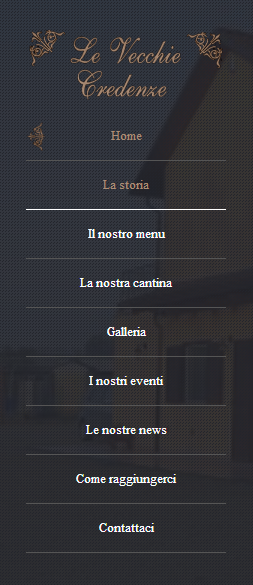
\includegraphics[width=0.4\textwidth]{images/navigation.png}
		\caption{Sezione navigation}
\end{figure}

\begin{figure}[H]
		\centering 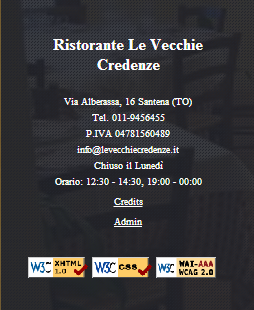
\includegraphics[width=0.4\textwidth]{images/footer.png}
		\caption{Sezione occupata dal footer}
\end{figure}

\paragraph{Content}

Questa sezione invece contiene i contenuti veri e propri presentati nelle pagine del sito, introdotti sempre da un titolo.

\begin{figure}[H]
		\centering 
\includegraphics[width=0.4\textwidth]{images/content.png}
		\caption{Sezione dedicata ai contenuti}
\end{figure}

\subsection{L’utilizzo delle mediaquery}

Per affrontare il problema della intercompatibilità tra le varie piattaforme abbiamo utilizzato le mediaquery che linkano ai diversi CSS adattati alle dimensioni dello screen della piattaforma stessa da cui si sta effettuando l’accesso al sito.
Le diverse piattaforme individuate sono:
\begin{itemize}
\item Desktop, a cui si collega screen.css;
\item Tablet, a cui si collega tablet-landscape.css;
\item Smartphone, a cui si collegano smartphone-portrait.css e smartphone-landscape.css;
\item Stampa, a cui si collega print.css
\end{itemize}

\subsection{I colori}

\paragraph{Background}

Per la visualizzazione della pagina a schermo intero abbiamo utilizzato una slide show di immagini mentre per le versioni per tablet e smartphone questa è stata rimpiazzata da uno sfondo monocromatico per rendere più leggera e chiara la visualizzazione dei contenuti.

\paragraph{Link}

Per i link del campo content si è deciso di scegliere un colore oro per i link visitati mentre per i selected abbiamo mantenuto il colore “standard” del sito che riprende stilisticamente il banner presente in navigation. Per quanto riguarda i link del menu presente in navigation abbiamo deciso, pur essendo consapevoli del fatto che al fine di rendere un sito accessibile sarebbe opportuno cambiare il colore dei link visitati anche al menu di navigazione, di mantenere un colore classico (bianco) per evitare confusione o effetti spiacevoli alla vista poiché il principale obbiettivo è di creare una vetrina per un ristorante quindi deve essere quanto più piacevole alla vista possibile. 

\begin{figure}[H]
		\centering 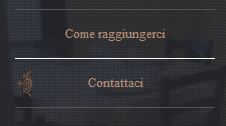
\includegraphics[width=0.4\textwidth]{images/link-navigation.png}
		\caption{Link della sezione navigation}
\end{figure}

\begin{figure}[H]
		\centering 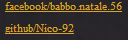
\includegraphics[width=0.4\textwidth]{images/link-content.png}
		\caption{Effetto per i link visistati presenti nel content}
\end{figure}

\subsection{CSS3}

Le proprietà del nuovo standard che abbiamo utilizzato nel nostro progetto sono:

\paragraph{Background-size}

Utilizzato per regolare la grandezza delle immagini di background  della slide show e del banner.

\paragraph{Border- radius}

Utilizzato per arrotondare i margini nella sezione social e nelle immagini della sezione credits.

\paragraph{box-shadow}
Questa proprietà è stata implementata nei form della parte di amministrazione, qualora l' amministratore cerchi di eseguire l' input di un form avendo lasciato dei campi obbligatori vuoti, tali campi verranno evidenziati con un' aura rossa abbastanza evidente in modo da essere anche accessibile.
\begin{figure}[H]
		\centering 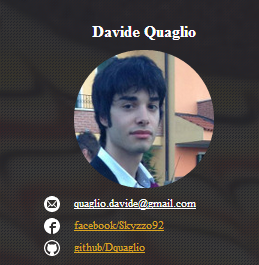
\includegraphics[width=0.5\textwidth]{images/radius.png}
		\caption{Utilizzo della proprietà radius nella pagina Contattaci}
\end{figure}

\paragraph{Si ricorda che}

Abbiamo inoltre utilizzato la proprietà webkit che non è parte attualmente degli standard css ma gli ultimi aggiornamenti del validatore w3c hanno declassato tali errori a warning, e si sta valutando di aggiungere webkit allo standard.

\begin{figure}[H]
		\centering 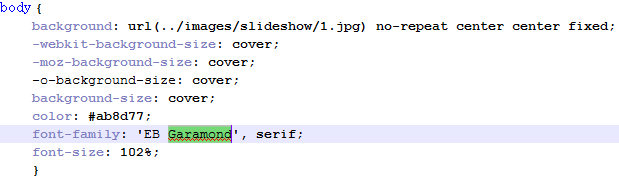
\includegraphics[width=0.4\textwidth]{images/webkit.png}
		\caption{Utilizzo della proprietà webkit nel Body}
\end{figure}

\subsection{Note importanti}

\paragraph{Font}

Abbiamo scelto di utilizzare un font più elaborato (Garamond) poiché il sito è creato come vetrina per un ristorante e quindi abbiamo privilegiato l’immagine e l’impatto estetico a scapito dei tempi di caricamento delle pagine stesse anche se la differenza in velocità è pressoché impercettibile.
